\documentclass[a4paper,12pt]{article}

%%% Работа с русским языком
\usepackage{cmap}					% поиск в PDF
\usepackage{mathtext} 				% русские буквы в фомулах
\usepackage[T2A]{fontenc}			% кодировка
\usepackage[utf8]{inputenc}			% кодировка исходного текста
\usepackage[english,russian]{babel}	% локализация и переносы
\usepackage{float}
%%% Дополнительная работа с математикой
\usepackage{amsfonts,amssymb,amsthm,mathtools} % AMS
\usepackage{amsmath}
\usepackage{setspace}
\usepackage{icomma} % "Умная" запятая: $0,2$ --- число, $0, 2$ --- перечисление

%% Номера формул
%\mathtoolsset{showonlyrefs=true} % Показывать номера только у тех формул, на которые есть \eqref{} в тексте.

%% Шрифты
\usepackage{euscript}	 % Шрифт Евклид
\usepackage{mathrsfs} % Красивый матшрифт

%% Свои команды
\DeclareMathOperator{\sgn}{\mathop{sgn}}

%% Перенос знаков в формулах (по Львовскому)
\newcommand*{\hm}[1]{#1\nobreak\discretionary{}
	{\hbox{$\mathsurround=0pt #1$}}{}}

%%% Работа с картинками
\usepackage{graphicx}  % Для вставки рисунков
\graphicspath{{images/}{images2/}}  % папки с картинками
\setlength\fboxsep{3pt} % Отступ рамки \fbox{} от рисунка
\setlength\fboxrule{1pt} % Толщина линий рамки \fbox{}
\usepackage{wrapfig} % Обтекание рисунков и таблиц текстом

%%% Работа с таблицами
\usepackage{array,tabularx,tabulary,booktabs} % Дополнительная работа с таблицами
\usepackage{longtable}  % Длинные таблицы
\usepackage{multirow} % Слияние строк в таблице
\usepackage[unicode, pdftex]{hyperref}
\usepackage{xcolor}
\definecolor{urlcolor}{HTML}{0000ff}
\definecolor{linkcolor}{HTML}{030134}
\hypersetup{pdfstartview=FitH,  linkcolor=linkcolor,urlcolor=urlcolor, colorlinks=true}
%%% Заголовок
\author{Владимир Димитров \\ email: v.dimitrov@g.nsu.ru}
\title{Описание работы}
\date{\today}

\begin{document}
	\maketitle
	\newpage
	\tableofcontents
	\newpage
	\section{Данные}
	Набор данных \href{https://github.com/karolpiczak/ESC-50}{ESC-50} представляет собой размеченную выборку из 2000 записей окружающей среды. Набор данных состоит из 50 классов, которые можно распределить по 5 главным категориям:
	\begin{enumerate}
		\item Животные
		\item Звуки природы
		\item Звуки человека
		\item Бытовые звуки
		\item Звуки города
	\end{enumerate}
	Для каждого из класса доступно по 50 наблюдений. Давайте обучать наш классификатор предсказывать один из 50 классов. Для этого сначала необходимо удобно представить данные, потом найти подходящую архитектуру, используя статьи или посты в интернете.
	
	\section{Классы}
	
	\subsection{TaskConfig}
	Для удобной работы с кодом создадим класс TaskConfig, в котором есть возможность  редактирования параметров как модели, так и данных. Он умеет создавать вавку более длинной (за это отвечает переменная n\_mels), можно поиграться с длиной батча и шагом обучения (learning\_rate, batch\_size). 'Ужать' нашу модель с помощью параметра регуляризации (weight\_decay), выбрать размер тренировочной выборки и многое другоe.
\begin{figure}[H]
	\centering
	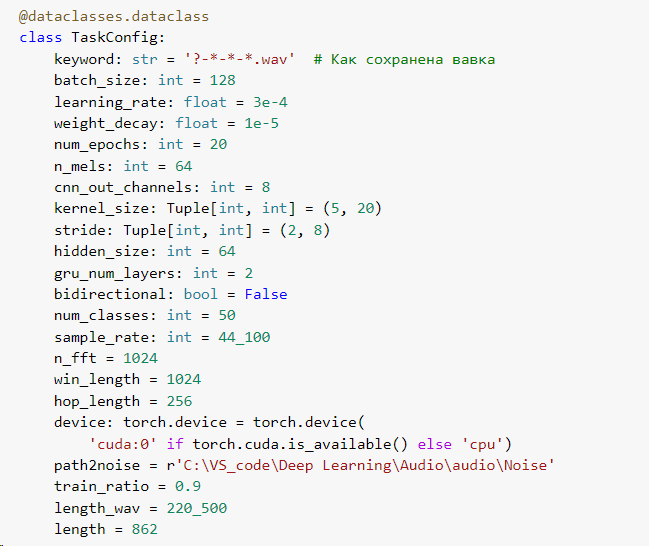
\includegraphics[width=0.9\linewidth]{Image/Taskconfig}
	\caption{Реализация класса TaskConfig}
	\label{fig:taskconfig}
\end{figure}
	
	Более подробное описание представлено в главе \ref{TaskConfig}.

 	
 	\subsection{Dataset}
 	\begin{figure}[H]
 		\centering
 		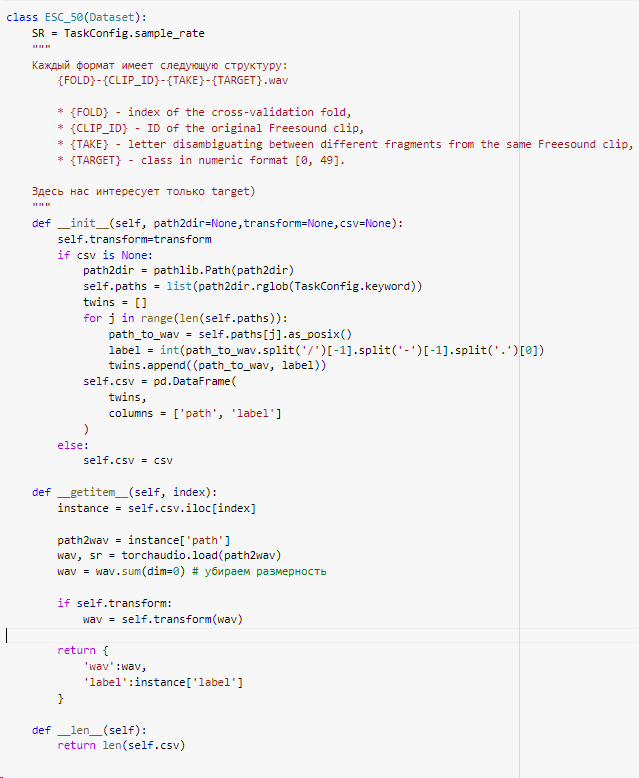
\includegraphics[width=0.7\linewidth]{Image/Dataset}
 		\caption{Реализация класса ESC\_50}
 		\label{fig:dataset}
 	\end{figure}
 	
 	Данный класс имеет типичную структуру: метод get и метод len. Get вызывает элемент соответствующего индекса, а метод len возвращает длину. Из интересного - это инициализатор, в который подается путь до наших файлов, а он находит метки класса (необходимо чтобы они были в имени файла) и создает csv файл с двумя колонками: путь до файла и метка класса.
 	
  Более подробное описание представлено в главе \ref{ESC50}.
  
 	\subsection{Augmentation}
		\begin{figure}[H]
			\centering
			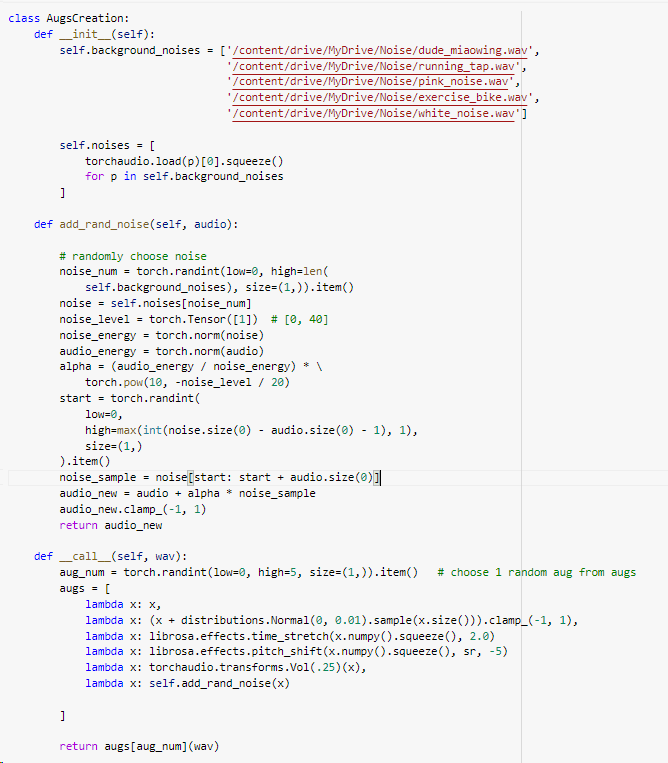
\includegraphics[width=0.7\linewidth]{Image/Augmentation2}
			\caption{Реализация класса Augmentation}
			\label{fig:augmentation2}
		\end{figure}

 	 
 	 Класс Augmentaion реализован на примере \href{https://towardsdatascience.com/audio-deep-learning-made-simple-part-3-data-preparation-and-augmentation-24c6e1f6b52}{статьи}. В данном классе есть 5 различных видов аугментации: 
 	 
 	 \begin{itemize}
 	 	\item Gaussian Noise - довольно простой метод аугментации, связан с добавлением случайной величины распределенной нормально. 
 	 	\item Time Stretching - ускорение вавки. Можно использовать наивный подход и брать каждый второй элемент нашей вавки, а можно использовать библиотеку librosa (Для более подробного ознакомления читать здесь \cite{2}).
 	 	\item Pitch Shifting - эта аугментация изменяет высоту голоса. Например, трансформация, которая представлена в классе делает голос более "тяжелым".
 	 	\item Volume - увеличивает уровень громкости.
 	 	\item Noise - добавляет случайные звуки
 	 \end{itemize}
  	
  	Еще существуют аугментации, которые накладываются на MEL-спектограммы, в статье \cite{1} подробно рассказываются как их можно реализовать. Также есть интересный \href{https://speechbrain.readthedocs.io/en/latest/API/speechbrain.processing.speech_augmentation.html#speechbrain.processing.speech_augmentation.AddBabble}{модуль}. 
 	 
 	\subsection{Collator}
 	
 	\begin{figure}[H]
 		\centering
 		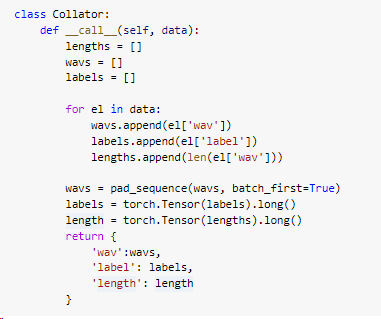
\includegraphics[width=0.7\linewidth]{Image/Collator}
 		\caption{Реализация класса Collator}
 		\label{fig:collator}
 	\end{figure}
 	Данный класс необходим для удобного обращения с данными. Через него можно указывать модели по какой переменной обучаться, по какой считать лосс, а по какой нормализовать (если это требуется).
 	
 	
 	\subsection{Формирование данных}
 	\begin{figure}[H]
 		\centering
 		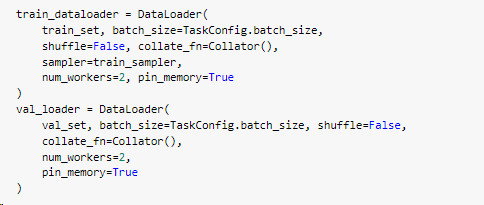
\includegraphics[width=0.7\linewidth]{Image/Dataloader}
 		\caption{Создание датасетов}
 		\label{fig:dataloader}
 	\end{figure}
 
 	В DataLoader подаем наши данные, которые мы сначала обработали с помощью класса ESC-50. Sampler необходим для несбалансированной выборки, он пересчитывает веса в зависимости от количества наблюдений одной метки, которые попали в train (Реализация данной функции представлена в главе \ref{getsampler}).
 	Шафл не производится, так как индексы по которым мы доставали наши данные - случайны. Переменная pin\_memory оптимизирует работу нашей модели путем резервирования памяти (Более подробно можно почитать \href{https://medium.com/deelvin-machine-learning/pytorch-performance-tuning-in-action-7c4d065d4278}{здесь}).
	\subsection{Featurizer}
		\begin{figure}[H]
			\centering
			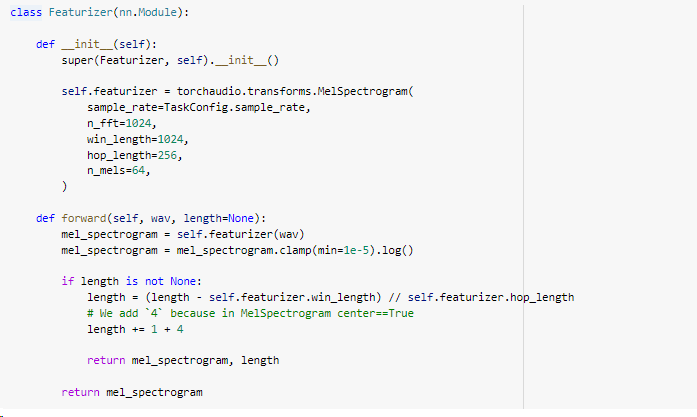
\includegraphics[width=0.7\linewidth]{Image/Featurizer}
			\caption{Реализация класса Featurizer}
			\label{fig:featurizer}
		\end{figure}
		Данный класс трансформирует нашу вавку и переводит ее в Mel-спектрограмму (Более подробно о Mel-спектограмме \href{https://medium.com/analytics-vidhya/understanding-the-mel-spectrogram-fca2afa2ce53}{здесь}). Сам алгоритм будет на вход получать вавку, которую мы пропустили через класс Featurizer. Из интересного, это нормализация вавки в зависимости от ее длины. Так как в реальной жизни, скорее всего, данные имеют разную длину, то конкретно данная фитча явялется достаточно полезным дополнением. Почитать более подробно про класс можно в главе \ref{Featurizer}
		
	
		 	
\section{Model}

\textbf{Замечание:} В дальнейшем все модели будут обучаться на 10 эпохах. Это связано с вычислительными мощностями, которые в Google Colab строго регламентируются. Обучение будет происходить на основе CrossEntropy loss. Оптимизатор будет - Adam. Другие параметры модели можно найти в классе TaskConfig (\ref{TaskConfig}).
	\subsection{Baseline}
		
	\begin{figure}[H]
		\centering
		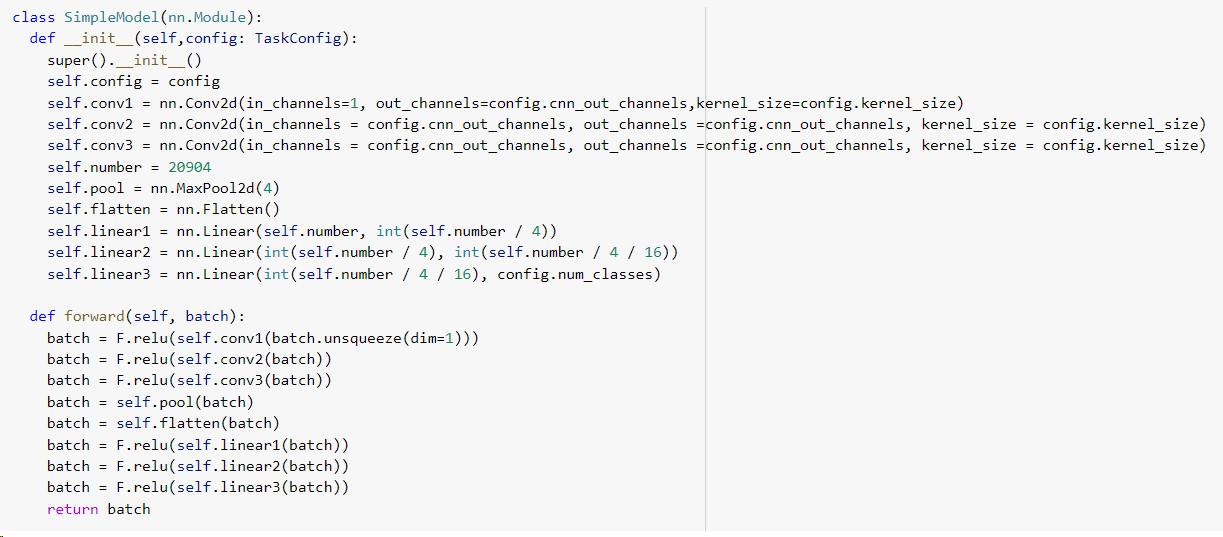
\includegraphics[width=1\linewidth]{Image/Simple_model}
		\caption{Baseline model}
		\label{fig:simplemodel}
	\end{figure}

	
	Давайте рассмотрим достаточно простую архитектуру, которую будем считать в качестве безлайна. 
	\begin{enumerate}
		\item VGG блок с 8 каналами. В него входят 3 сверточных слоя с ядром 3*3 и нелинейностью ReLU. Перед входом в линейный слой применяется Max pooling с ядром 4*4
		\item 3 полносвязных слоя между которыми применяется нелинейность ReLU.		
	\end{enumerate}
		\begin{figure}[H]
		\centering
		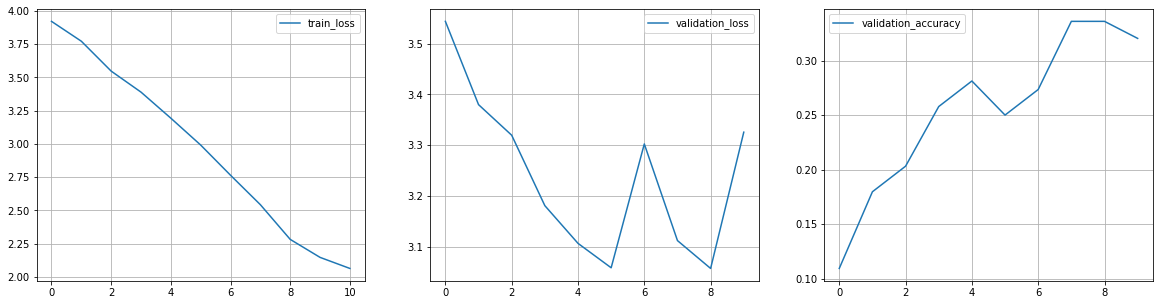
\includegraphics[width=1.2\linewidth]{Image/Baseline_train.png}
		\caption{Результаты базовой модели}
		\label{fig:featurizer1}
	\end{figure}
	Как видим потенциал у модели достаточно неплохой, на валидации точность составила порядка 33 процента. 
	\subsection{AdvancedModel}
		Особенность VGG блока заключается в том, что повышение качества работы сети достигается за счет увеличения числа последовательных блоков. При этом число фильтров в каждом новом блоке в 2 раза больше, чем в предыдущем. Усложним нашу модель, используя также \textbf{Dropout} и \textbf{Batch Normalize}.
		
		Правда сравнивать такие архитектуры достаточно не корректно, ведь для более глубоких сетей необходимо большее число эпох. Так как мощностей все также мало, мы докрутим шаг.
	\begin{figure}[H]
		\centering
		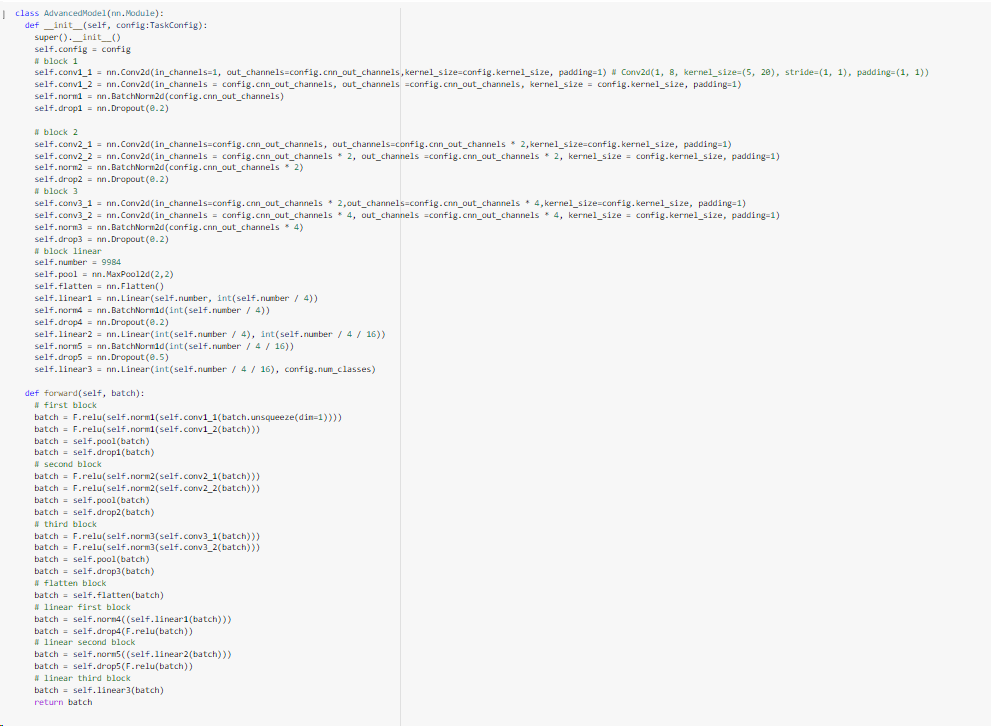
\includegraphics[width=1\linewidth]{Image/Advanced_model}
		\caption{Реализация улучшенной модели}
		\label{fig:advancedmodel}
	\end{figure}
	
	\begin{figure}[H]
	\centering
	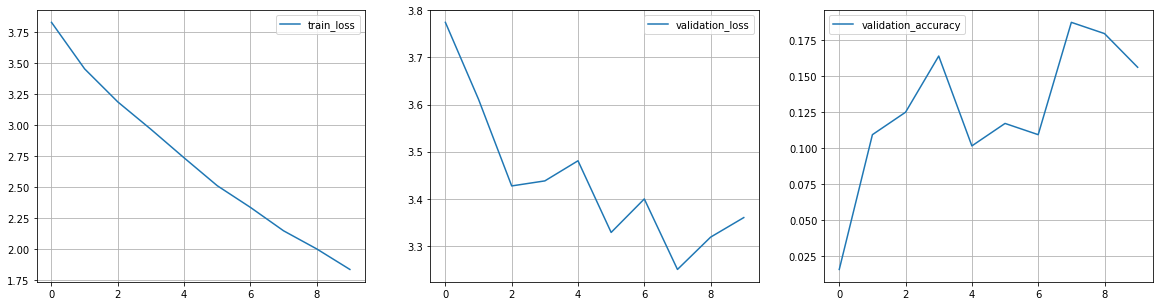
\includegraphics[width=1.2\linewidth]{Image/Advanced_model_train.png}
	\caption{Результаты улучшенной модели}
	\label{fig:featurizer1}
	\end{figure}
	Как мы видим, увеличение шага в два раза не спасло и модель недообучилась, поэтому необходимо в дальнейшем увеличить шаг еще больше или брать большее количество эпох. 
 	\subsection{LSTM}
 	Давайте рассмотрим рекуррентные нейронные сети c долгосрочной памятью, возьмем однослойнную LSTM (\href{https://medium.com/@premtibadiya/music-genre-classification-using-rnn-lstm-1c212ba21e06}{Идейный вдохновитель}). Преимущество данной сети в том, что она может аккумулировать прошлую информацию, которая  находится на достаточно дальнем расстоянии. 
 	\begin{figure}[H]
 		\centering
 		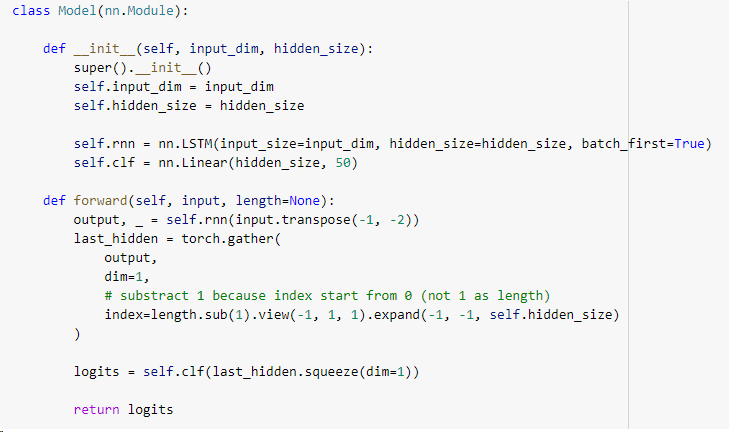
\includegraphics[width=0.7\linewidth]{Image/Featurizer1}
 		\caption{Реализация LSTM}
 		\label{fig:featurizer1}
 	\end{figure}
	
	Из интересных особенностей, здесь был использован torch.gather, который позволяет быстрее доставать индексы из тензора, нежели, чем это делать через обычные команды pythona (Почитать более подобно про torch.gather можно \href{https://medium.com/@mbednarski/understanding-indexing-with-pytorch-gather-33717a84ebc4}{здесь}).
 
 
 	\begin{figure}[H]
 	\centering
 	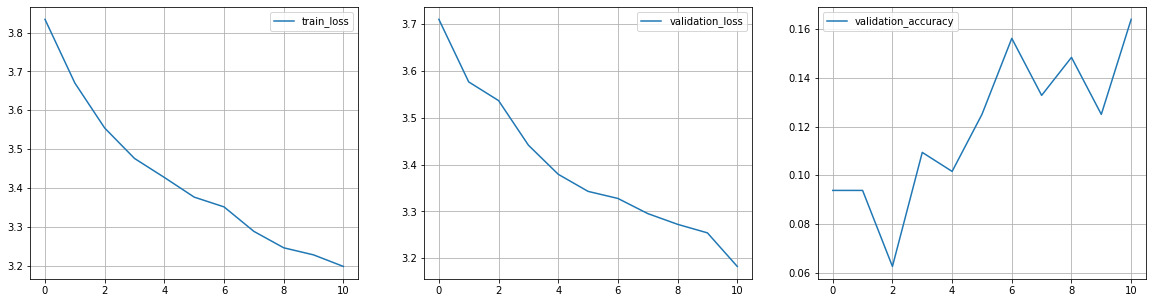
\includegraphics[width=1\linewidth]{Image/LSTM_train.png}
 	\caption{Результаты LSTM}
 	\label{fig:featurizer1}
 \end{figure}
	Данная модель хоть и не является глубокой (поэтому сравнение будет корректно), но она показала более худший результат на тех же 10 эпоха обучения, по сравнению с базовой моделью. Возможно информация, которая получает сеть из более ранних слоев, не содержит никаких полезных свойств, а возможно необходимо добавить сверточные слои, которые хорошо себя показали у базовой модели. Это имплементация будет реализована дальше.

	\subsection{CRNN-A}
	
	Данная архитектура объединяет несколько моделей в себе. Она использует:
	\begin{itemize}
		\item рекуррентные нейронные сети, которые позволяют агрегировать информацию в различные периоды времени.
		\item сверточные сети, которые позволяют улавливать сложные закономерности.
		\item механизм внимания, который позволяет сконцентрироваться на более значимых признаках.
	\end{itemize}
	
	\begin{figure}[H]
		\centering
		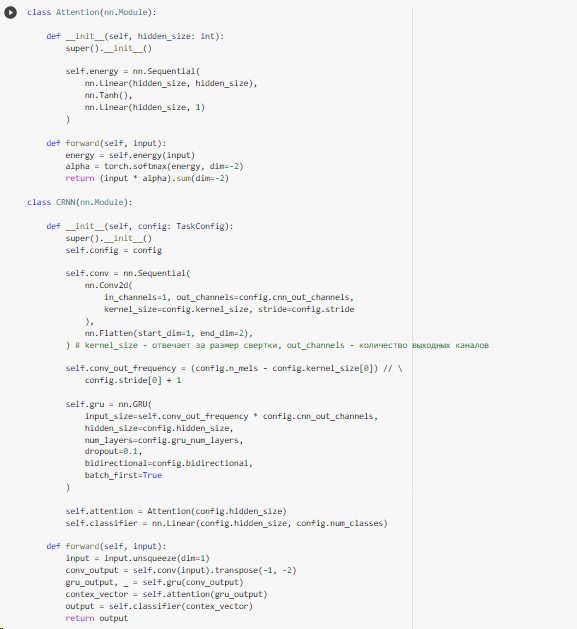
\includegraphics[width=1\linewidth]{Image/CRNN}
		\caption{CRNN-A модель}
		\label{fig:crnn}
	\end{figure}
	
 	\begin{figure}[H]
 		\centering
 		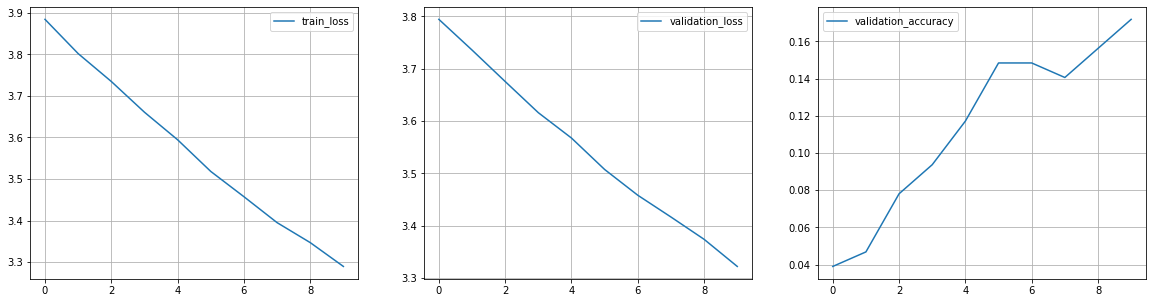
\includegraphics[width=1\linewidth]{Image/CRNN_train.png}
 		\caption{Результаты CRNN модели}
 		\label{fig:crnn}
 	\end{figure}
 
 	Все результаты необходимо воспринимать достаточно условно, ведь модели не успевают научиться обобщать наши данные. Поэтому стоит ее обучать чуть дольше, но так как вычислительных мощностей мало, давайте обратимся уже к предобученной модели.
	 	
 	\subsection{Transfer learning: VGG19}
 	В библиотеке torchvision имплементировано не только большое множество моделей (всевозможные ResNet'ы, Inception, VGG, AlexNet, DenseNet, ResNext, WideResNet, MobileNet...), но и загружены чекпоинты обучения этих моделей. Однако, из всей этой роскоши, нам понадобится только одно: модель VGG. Заменим 1 слой и последний для соответствия размерности.
 		\begin{figure}[H]
 		\centering
 		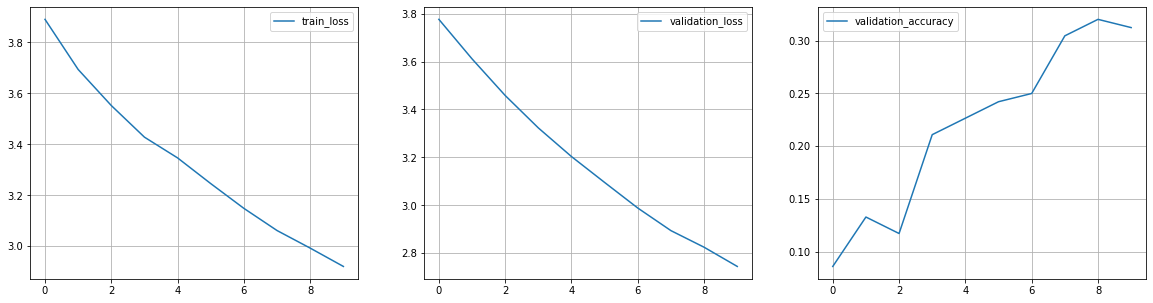
\includegraphics[width=1\linewidth]{Image/Transfer_learning_results.png}
 		\caption{Результаты VGG19}
 		\label{fig:crnn}
 	\end{figure}
 	Обученная модель показала производительность на уровне baseline модели, возможно, это связано с тем, что модель изначально обучалась на ImageNet данных, поэтому ей необходимо чуть больше времени на донастройку параметров.
 	\subsection{Github model}
 	Код был взят  \href{https://github.com/anuragkr90/weak_feature_extractor}{отсюда}. Код написан по статье \cite{5}. Структура достаточно тривиальна, она вбирает в себя достаточно много сверток, которые на каждом шагу пулятся и от них берется нелинейность. 
 	\begin{figure}[H]
 		\centering
 		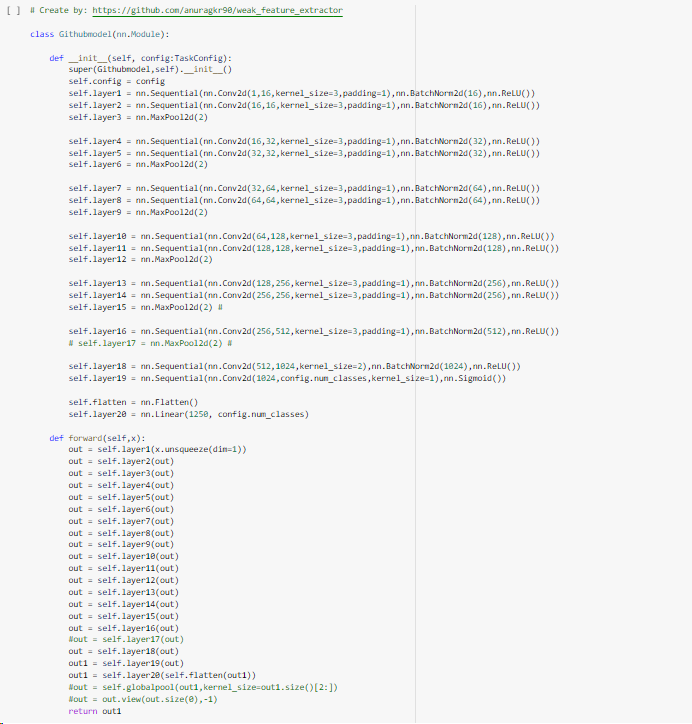
\includegraphics[width=0.7\linewidth]{Image/Github_model}
 		\caption{Github model}
 		\label{fig:githubmodel}
 	\end{figure}
 
 		\begin{figure}[H]
 		\centering
 		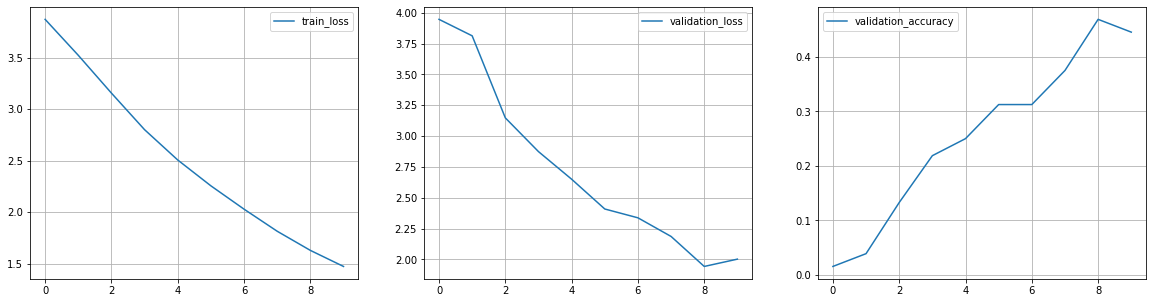
\includegraphics[width=1\linewidth]{Image/Github_model_train.png}
 		\caption{Результаты Github model}
 		\label{fig:githubmodel}
 	\end{figure}
 Данная структура показала лучшую производительность среди необученных архитектур. На последней эпохе точность составила 42 процента. Автор статьи утверждает, что лучший результат составил 81 процент!
 	\newpage
 	
 	\section{Вывод}
 	Лучше всего из рассмотренных архитектур показали себя сверточные нейронные сети. Возможно, это связано с тем, что мы по сути предсказываем метку по Mel-спектрограмме, а последняя в свою очередь является ничем иным, как картинкой. А сверточные сети как раз хорошо работают именно с картинками. Также достаточно полезной была техника  аугментации, кодирования весов в зависимости от количества классов, попадающих в тренировочную выборку, применения dropout и нормализации. В дальнейшем хотелось бы реализовать архитектуры, связанные с трансформерами, попробовать ML модели и поработать с более 'живыми' данными. 
 	\newpage
 	
 	 	\section{Приложение}
 	
 	\subsection{Описание класса TaskConfig}\label{TaskConfig}
 		\begin{itemize}
 		\item $keyword$ - способ сохранения аудио, например: 'АBC-31-31-32.wav' в переменную надо подать '?-*-*-*.wav'
 		\item $batch\_size$ - сколько данных попадет в батч
 		\item $learning\_rate$ - длина шага обучения
 		\item $weight\_decay$ - параметр регуляризации
 		\item $num\_epochs$ - количество эпох обучения
 		\item $n\_mels$ - количество мелов, на которые будет разбита вавка (влияет на размер входного тензора)
 		\item $cnn\_out\_channels$ - количество каналов выходов для сверточного слоя
 		\item $stride$ - длина шага
 		\item $hidden\_size$ - размер скрытого слоя
 		\item $gru\_num\_layers$ - число рекуррентных слоев
 		\item $bidirectional$ - создание двунаправленной рекуррентной сети
 		\item $num\_classes$ - число классов для предсказания
 		\item $sampel\_rate$ - частота дискретизации
 		\item $device$ - девайс на котором будут производиться расчеты
 	\end{itemize}
 	
 	\subsection{Описание класса ESC\_50}\label{ESC50}
 		\begin{itemize}
 		\item $\_\_init\_\_$ - подается путь до файла, в данном методе создается файл csv, для более удобного представления данных. Также возможна применение аугментации (в переменной transform)
 		\item $\_\_getitem\_\_$ - возвращает объект из csv файла по указанному индексу и применяет (если указано) аугментацию. На выходе возвращает словарь состоящий из тензорного представления вавки и метки класса
 		\item $\_\_len\_\_$ - возвращает длину нашего csv файла
 	\end{itemize}
 	\subsection{Get\_sampler}\label{getsampler}
 	\begin{figure}[H]
 		\centering
 		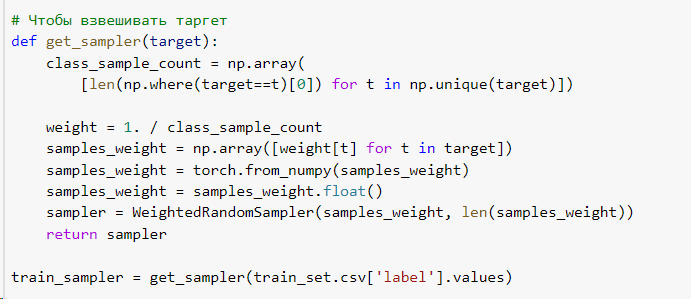
\includegraphics[width=0.7\linewidth]{Image/Get_sampler}
 		\caption{Реализация функции get\_sampler}
 		\label{fig:getsampler}
 	\end{figure}
 	
 	
 	\subsection{Описание класса Featurizer}\label{Featurizer}
 		\begin{itemize}
 		\item n\_fft - количество амплитуд, на которые мы раскладываем вавку
 		\item win\_length - окно, с которым мы вырезаем вавку
 		\item hop\_length - длина шага, на которую мы сдвигаемся
 		\item center - переменная, которая отвечает за паддинг тишины.В статьях написано, что введение данной переменной необходимо для того, чтобы не потерять начало сигнала из-за окна
 		\item onesided - одно из свойств спектрограммы ее симметричность, данная функция возвращает только одну сторону (отрезает половину амплитуд).
 		\item n\_mels - параметр сжатия, отвечает за конечную размерность данных
 		\item window\_fn - окно, которое сглаживает нашу спектрограмму.
 	\end{itemize}
 
 	\subsection{Github}
 	\begin{spacing}{2}
 		{\Large
 			\href{https://github.com/Vladimir-Dimitrov-Ngu/Audio_DL/tree/master/Work/Code}{Code}}
 	
 	\end{spacing}
 	
 	
 	
 	
 	\newpage
\begin{thebibliography}{9}
	
	\bibitem[1]{1}Park D. S. et al. Specaugment: A simple data augmentation method for automatic speech recognition //arXiv preprint arXiv:1904.08779. – 2019.
	\bibitem[2]{2} De Götzen A., Bernardini N., Arfib D. Traditional implementations of a phase-vocoder: The tricks of the trade //Proceedings of the COST G-6 Conference on Digital Audio Effects (DAFX-00), Verona, Italy. – 2000.
	\bibitem[3]{3}Tian C., Ji W. Auxiliary multimodal LSTM for audio-visual speech recognition and lipreading //arXiv preprint arXiv:1701.04224. – 2017.
	
	\bibitem[4]{4} Shan C. et al. Attention-based end-to-end models for small-footprint keyword spotting //arXiv preprint arXiv:1803.10916. – 2018.
	
	\bibitem[5]{5}Kumar A., Khadkevich M., Fügen C. Knowledge transfer from weakly labeled audio using convolutional neural network for sound events and scenes //2018 IEEE International Conference on Acoustics, Speech and Signal Processing (ICASSP). – IEEE, 2018. – С. 326-330.
\end{thebibliography} 
 	
\end{document}
